\myexternaldocument{blockchain}
\subsection{Ethereum}
{
Ethereum motivation was to leverage the first blockchain networks, such as Bitcoin, and overcome their constraints. In a nutshell, Ethereum is a blockchain that works like a computer embedded, so is prepared to run apps and organizations in a decentralized, permissionless and censorship-resistant way.

In Ethereum, we can talk about a single computer called \acrfull{evm} that establishes which is the state that every node on the network should agree on. Any participant can broadcast a request for \acrshort{evm} to perform a computation over the state. When it happens, other participants on the network validate and ensure the request is signed by the address that sends it. If verified, then they check if that address has permission to execute the state change, if so they do it. Consequently, the state changes in the EVM and propagates throughout the network. Such requests for computations are called transaction requests and are stored on the blockchain by order along with the current state of the \acrshort{evm}. 

A "node" is any instance of Ethereum client software that is connected to other computers also running Ethereum software, creating a network. To read more information about the Ethereum client you can find it in appendix \ref{appendix:ethereum-client}.

Ethereum gathers a lot of concepts and the core ones are explained in the following sections. For more information, you can start by reading the original {Ethereum Whitepaper}\cite{ethereum-whitepaper}.
}

\subsubsection{Ethers}
{\acrfull{eth} is the native cryptocurrency of Ethereum and its purpose is to boost a market for computation. \acrshort{eth} represents an economic incentive for participants to provide computational resources to the network, which allows transactions to be validated and executed.

In Ethereum, when users want to make a transaction, they must pay some amount of \acrshort{eth} to the network as a bounty. These usage costs are known as gas fees. The network will award to the participant that eventually verifies the transaction, executes it and commits it to the blockchain.

This ``\gls{tip}" that senders pay, is equivalent to the amount required by the resources to carry out the computation and depends on the demand of computation power at that moment. Furthermore, paying an amount also prevents malicious participants from blocking the network by requesting infinite computation or other intensive tasks since they must pay for computation resources. If a task runs out of all the ether fees paid, the transaction gets terminated and the network returns to normal.

\acrlong{eth} can just be created on the creation of a new block process and is performed by the protocol definition, so any user can create. About 1/8 of the total issuance goes to the block proposer, whilst the remainder is distributed across the other validators. By contrast, \acrlong{eth} is destroyed on every transaction. This process is called ``burning'' and the removal is permanent. When users pay for their transactions a base gas fee is destroyed. This amount is defined by the blockchain according to the computation power demand.

The \acrshort{evm} stores the state, and this state is a ledger of all the accounts that have executed a transaction on the network. The final state provides us the current balance in \acrshort{eth} of all the accounts. Such accounts are able to send, hold and receive \acrshort{eth} from other accounts and interact with deployed smart contracts. We may find two types of accounts:
\begin{itemize}
    \item Externally-owned accounts (EOA), controlled by a person with the private key.
    \item Contract account, which is a smart contract deployed to the network and controlled by the code.
\end{itemize}
}

\subsubsection{Gas}
{Gas refers to the unit that measures the amount of computational effort required to execute specific operations on the Ethereum network. Each transaction to the network requires computation resources to execute. Such resources must be paid for to ensure Ethereum cannot get stuck in infinite computational loops. Note that regardless the transaction fails or succeeds the computation could have been carried out so the fee is paid in any case. Therefore, this gas fee appears to justify the payment for computation as is reflected in figure \ref{fig:gas-per-computation}.

\begin{figure}[H]
\centering
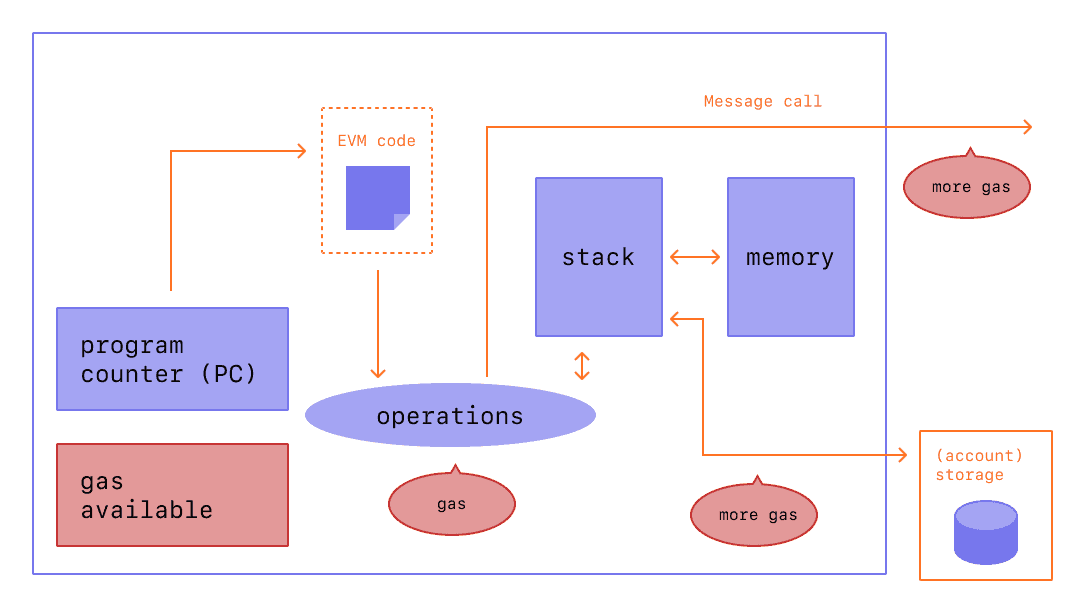
\includegraphics[width=12cm]{img/ethereum/gas.png}
\caption[Gas consumed per computation]{\footnotesize{Gas consumed per computation.}}
\label{fig:gas-per-computation}
\end{figure}

If we want to calculate the gas fee that a transaction requires we have to define it as the amount of gas used to do some operation, multiplied by the cost per unit gas. The \acrshort{evm} specifies the units of gas required by each computational operation \cite{opcodes-evm}. On the one hand, the base fee is set by the protocol depending on the number of blocks before it so it is easily predictable for users. On the other hand, the priority fee incentivizes validators to include a transaction on the block. The minimum amount of gas to pay is the base fee, but without a tip validators most likely will choose other transactions over yours or even create blocks with no transactions since they would receive the same award. So it is important to make this gas estimation predictable so users that offer too much waste some \acrshort{eth} or, by contrast, users that offer too little will not get a validator that chooses the transaction.  

Gas fees have to be paid in \acrshort{eth} and it is divided in two components: the \textbf{base fee} and the \textbf{priority fee} or \gls{tip}.


It is important to mention that users can define the maximum limit they are willing to pay for their transactions. This parameter is known as \textit{maxFeePerGas} and it must be greater than the sum of the base fee and the tip. The transaction sender is refunded with the difference between the max fee and the sum of the base fee and tip. This parameter is crucial because gas fees can get so high due to too much computation power demand or even complex smart contracts apps doing lots of operations.
}
\begin{figure}[H]
\centering
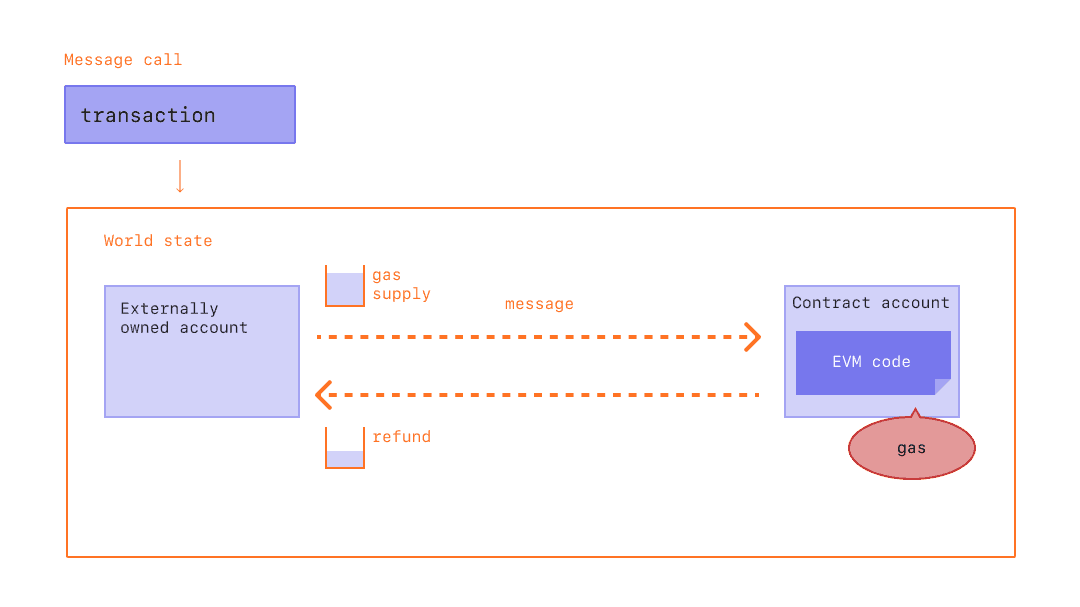
\includegraphics[width=12cm]{img/ethereum/gas-tx.png}
\caption[Gas refund procedure]{\footnotesize{Gas refund procedure.}}
\label{fig:gas-tx}
\end{figure}

{In brief, gas fees help to keep the Ethereum network secure. By requiring these bounties for computation it prevents bad actors from clogging the network. In addition, it also helps to avoid accidental loops or other intensive computational wastage in code.}


\subsubsection{Ethereum Virtual Machine (EVM)}
{The \acrlong{evm} is present at any block in the Ethereum's chain and it is in charge of defining the rules for computing a new valid state from block to block.

Ethereum is in essence a \textbf{distributed state machine}, in which state is a large database that holds not only all accounts and their respective balances but also a state machine. This state machine can execute arbitrary machine code and change between blocks according to a pre-defined set of rules defined by the \acrshort{evm}.

The state data structure that contains the large database is called a \textit{modified Merkle Patricia Trie}, which points to all addresses by hashes based on a single root hash such as the Merkle tree idea explained thoroughly in appendix \ref{appendix:merkle-tree}. This system lets to verify transactions in the network really fast and without the need for knowing all the content.

Ethereum is like a \textbf{state transition function} where given an input, the \acrshort{evm} returns a deterministic output. In terms of state, the expression would be \(Y(S, T)=S'\), where \textit{S} is a valid old state, \(T\) a handful of new valid transactions, \(Y(S, T)\) is the transition function and \(S'\) is the new valid state. 

Transactions are instructions from accounts signed beforehand which can be classified into two types: \textbf{message calls} and \textbf{contract creation}. The last type results in the creation of a new contract account containing compiled smart contract bytecode. Whenever a message call is addressed to this contract account the bytecode is executed.


\acrshort{evm} contains several pieces as you may see in figure \ref{fig:ethereum-node}. One of them is a \textbf{memory} which lives during execution by is no persisted between transactions. Nevertheless, contracts contain also a Merkle Patricia \textbf{storage} associated with the contract account as part of the global state. 

\begin{figure}[H]
\centering
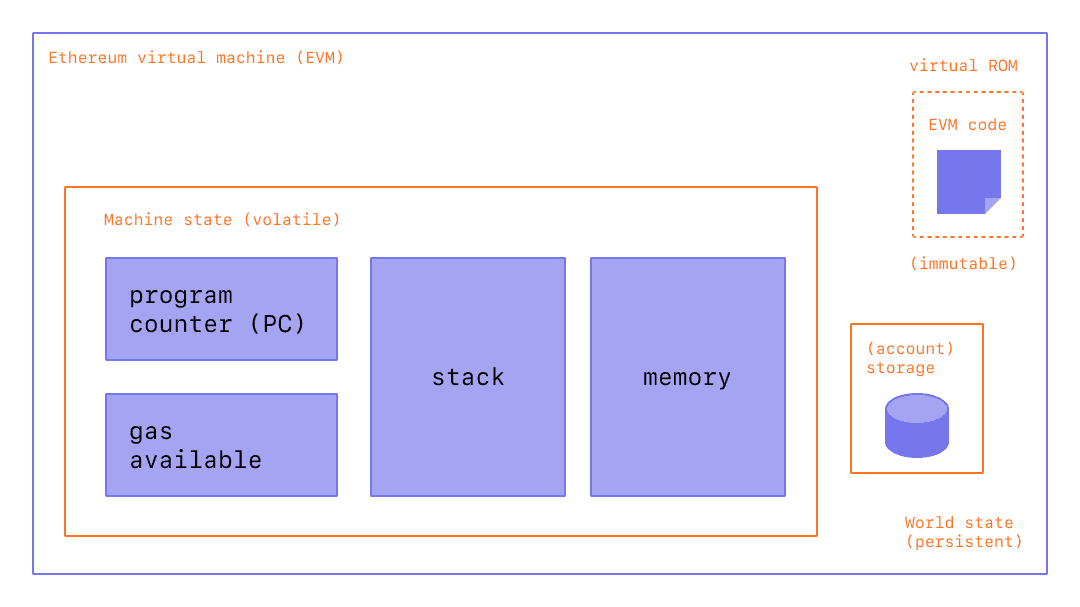
\includegraphics[width=12cm]{img/ethereum/evm.png}
\caption[Diagram of EVM internal components]{\footnotesize{Diagram of EVM internal components.}}
\label{fig:ethereum-node}
\end{figure}

Compiled smart contracts can perform standard stack operations such as {\small\textit{XOR, AND, ADD or SUB}}. In addition, \acrshort{evm} also implements some operations for blockchain purposes like {\small \textit{ADDRESS, BALANCE, BLOCKHASH}}, etc.

}

\subsubsection{Smart Contract}
{At this point, the power and potential of Ethereum is quite clear. The capability to add executable code within the state machine streamlines many recurrent tasks to the extent that developers no longer need to write new code each time they want to request a computation to the \acrshort{evm}. Instead, they can upload programs into the \acrshort{evm} state and make a request to them in order to execute those lines of code which may be configurable with varying parameters of the call. Those scripts uploaded and executed by the network are smart contracts.

One of the most explained analogies about a smart contract is a vendor machine. In a vendor machine, if you introduce correct inputs (money and snack selection), a certain output is guaranteed (snack is dispensed).

Deploying smart contracts is public. To do so, we just need to code a smart contract with some Ethereum developer language such as Solidity, the one chosen for this experiment. Such languages are compiled before being deployed so the \acrshort{evm} can understand the bytecode. Moreover, we need some \acrshort{eth} since deploy means to request a transaction, so we have to pay gas fees.

It is important to highlight a big constraint. They cannot get information about real-world events because the state machine needs to be deterministic and such events are happening off-blockchain. If we inject external data in the middle of a computation it will pollute security and decentralization so determinism could not be achieved. Likewise, using such external data really enhances the scope and value of smart contracts. So to solve it, data is introduced and stored in the blockchain by what is known as \textbf{oracles}. Once the data is recorded on the blockchain it can be consumed by smart contracts, but cannot be changed which ensures determinism is achieved.

In a nutshell, smart contracts are simply programs that run on the Ethereum blockchain. They can perform a set of actions, their functions, and handle data, their state, that is located to an Ethereum address, hence they have a balance and can receive and send transactions to any other address. This allows to call of other smart contracts that encourage composability.
}


\subsubsection{Decentralized Applications (dapps)}
{
What really empowers Web 3.0 are the decentralized applications. To define what is a decentralized application, we need to gather all the aforementioned concepts. A dapp is an application built on a decentralized network that combines smart contracts and a frontend user interface. Ethereum defines every smart contract as public, meaning transparent and accessible, hence any frontend application can interact with any smart contract, acting as an open \Gls{api}, even if you are not the owner of the smart contract.

If we think about how standard apps are implemented, we may define two isolated domains: frontend and backend. In the case of a dapp, the backend code runs on a decentralized peer-to-peer network like a blockchain instead of a centralized server. About the frontend, it could be written in any code like the apps do. If we focus on the hosting, the backend code is also hosted in the blockchain, whilst the frontend is not required, so it can be served from any centralized server. In practice, developers use web libraries such as ``\textit{ethers.js}"\cite{ethers} which will trigger and interact with the browser wallets like \textbf{Metamask}. Such wallets use \textbf{JSON RPC} protocol to connect through a public node, such as ``\textit{infura}"\cite{infura} or \textit{``geth"}\cite{geth}, to Ethereum and therefore, to the smart contract. This tech stack illustrated in figure \ref{fig:ethereum-node} is what conforms to a decentralized application.
}

\begin{figure}[H]
\centering
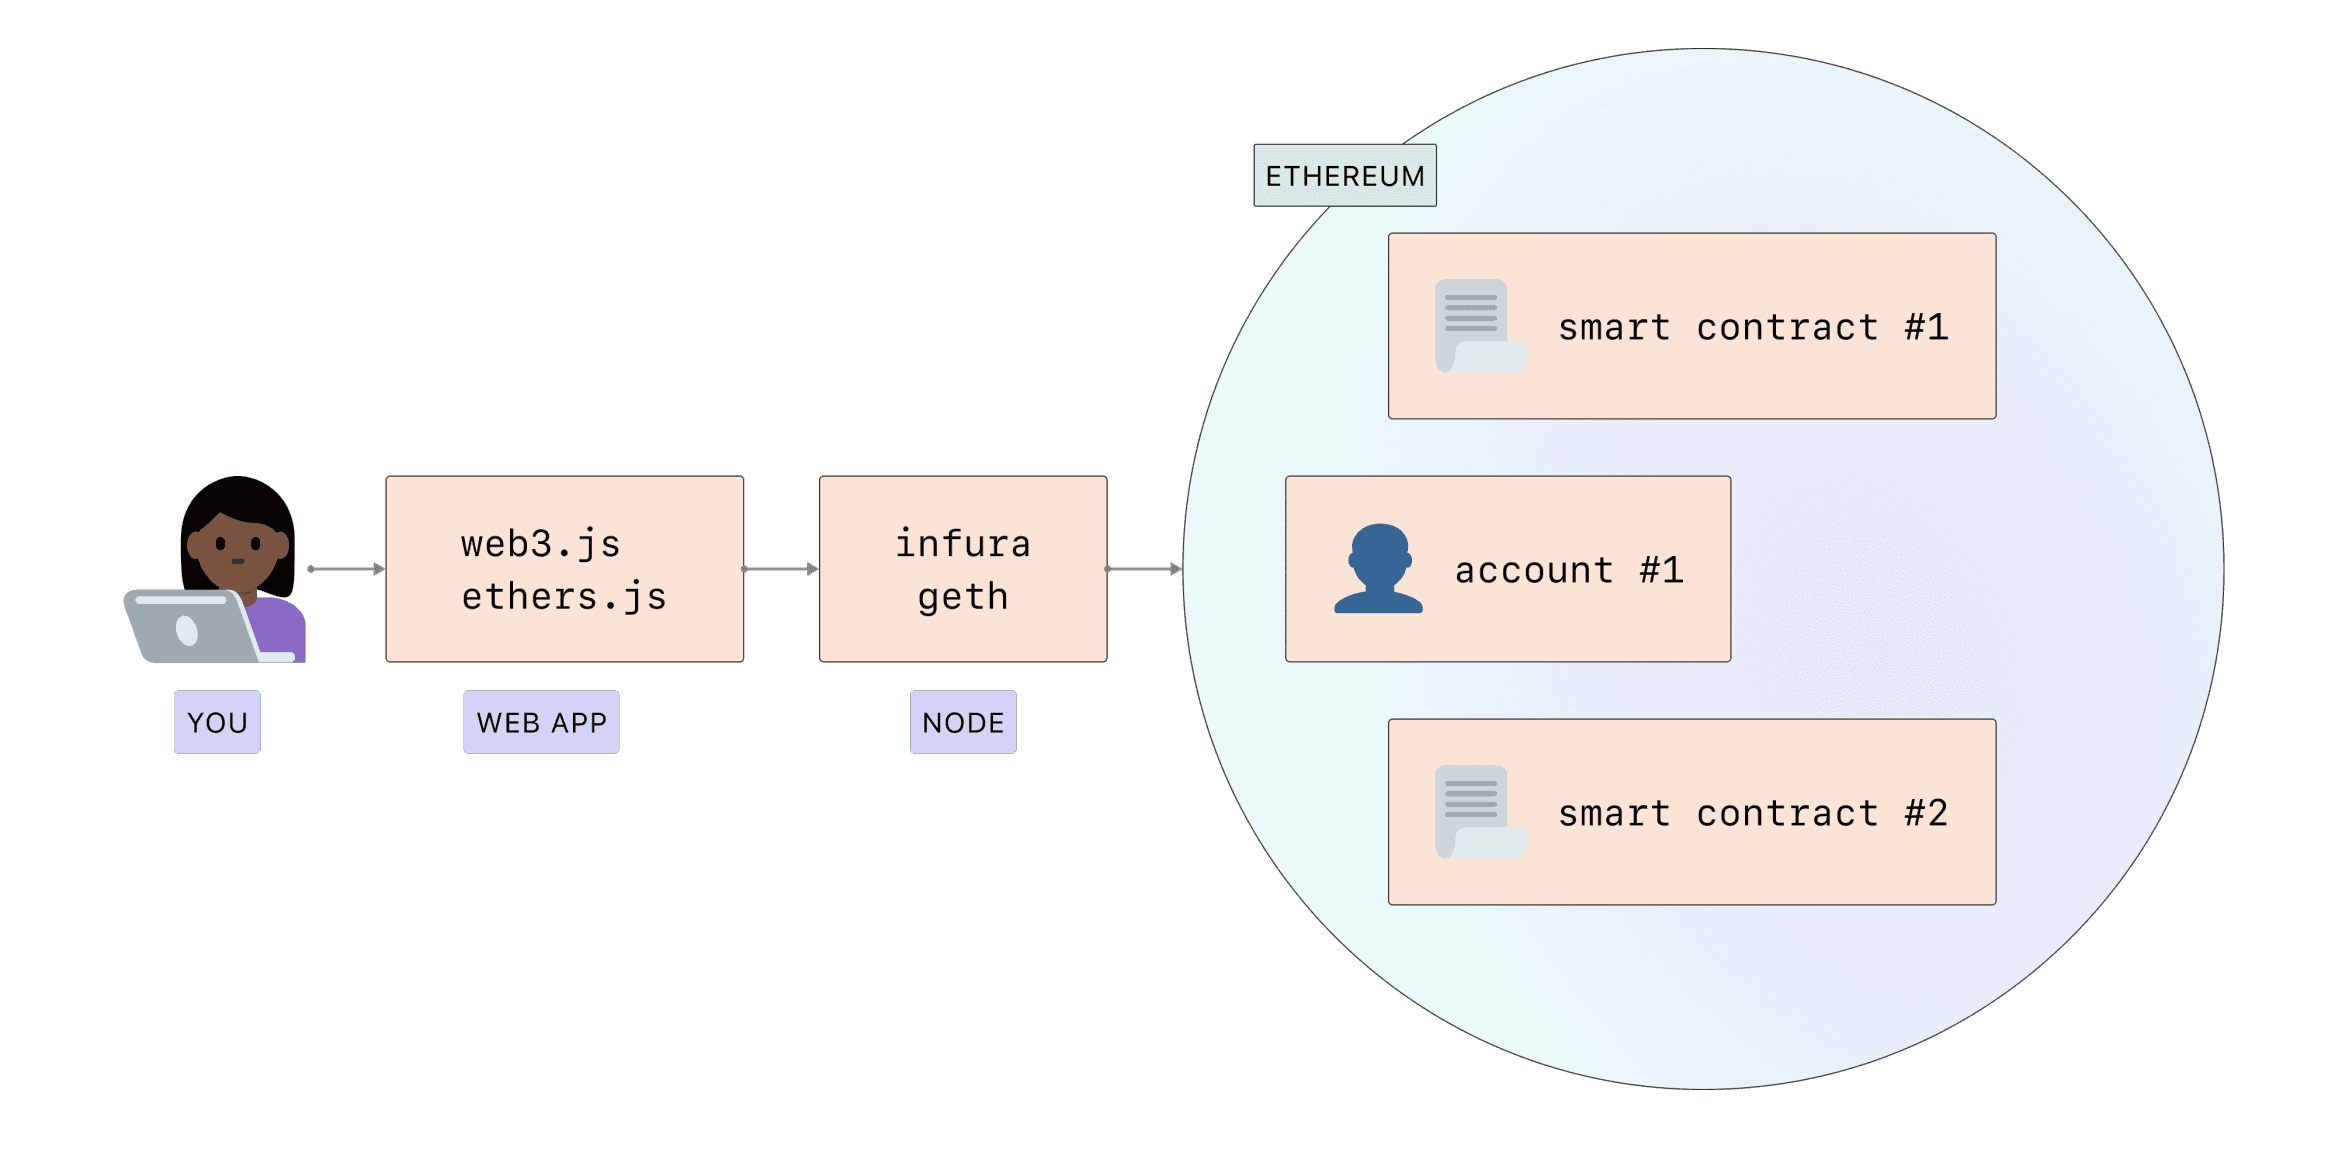
\includegraphics[width=14cm]{img/ethereum/nodes.png}
\caption[Ethereum connection from web applications]{\footnotesize{Ethereum connection from web applications}}
\label{fig:ethereum-node}
\end{figure}

{Dapps rely on their business logic in the network through the smart contracts, which run computations on the \acrlong{evm}. Such a code is always deterministic, meaning that given the same network state and the same input transaction, it is going to return the same output. It is also important to note that what is sent to the network cannot be changed so we must be very careful about the code that we write. It has bugs such as infinite loops or exhaustive processes that waste so much gas or even in the worst case security glitches, we could be able to update the code to fix them, so they must be designed and tested thoroughly. Opting for dapps provides some interesting benefits over usual applications but also has drawbacks that we must take into account. 

On the one hand, one of the most important advantages is the \textbf{zero downtime}. Since the code is deployed as a smart contract on the blockchain, the network will always be able to serve client requests so the service is never suspended. The blockchain wrapping also offers more \textbf{privacy} because the users will use address accounts to interact that are not linked to persons. In addition, dapps ensure \textbf{data integrity} on the blockchain. Such data is immutable and malicious actors cannot corrupt persisted information. Eventually, the more significant game changer properties are \textbf{censorship resistance} and 
\textbf{trustless behavior}. Smart contracts can be analyzed and predict what they will compute and return in a deterministic way, which completely replaces the need for trust in third parties with opaque processes. Moreover, no single entity can unilaterally block users from submitting transactions to change or read the state. This does not mean that we cannot define rules that allow just certain accounts to perform some actions but it must be coded in the moment of deployment. 

On the other hand, we may find some disadvantages to take into account, starting with \textbf{maintenance}, which requires complex solutions since we cannot modify the code once deployed. There is also a huge \textbf{performance overhead} because Ethereum demands that every node runs and stores each transaction and, in addition, \acrlong{pos} takes its time as well. Furthermore, there is a possibility of the network getting congested since it can only process 10-15 transactions per second, if the rate of transactions is greater than the capacity to process them or the computation required increases the mempools will be full of unconfirmed transactions. Eventually, if we take a look at the user experience consuming the dapp it can be penalized as well. Most end-users might find it difficult to understand the Ethereum basis and use this kind of tools that really leverages blockchain power. In favor of reducing this effect, software solutions built on top of the base layer of Ethereum might end up trusting part of the logic and data managed in centralized services which could eliminate partially the benefits of blockchain.

There is more detail about the Web evolution until the Web 3.0 model in the appendix \ref{appendix:web-evolution}.
}
